\chapter{排序的下界、線性時間排序與外部排序}
\label{ch:linear}

% 本章的圖共用的樣式。 敗者樹、勝者樹的圖由模擬程式依虛擬碼逐步執行後產生。
\tikzset{
    dtn/.style={draw=black!65, rounded corners=2pt, minimum width=0.95cm, minimum height=0.55cm, inner sep=1pt, font=\small},
    dtleaf/.style={draw=greenStroke, fill=greenFill, minimum height=0.55cm, inner sep=2pt, font=\small},
    dtbad/.style={draw=black!45, dashed, fill=black!4, minimum height=0.55cm, inner sep=2pt, font=\small, text=black!55},
    dte/.style={draw=black!60},
    dtpath/.style={draw=memStroke, very thick},
    lelab/.style={font=\scriptsize, text=black!65, inner sep=1pt},
    lte/.style={draw=black!60},
    ltn/.style={circle, draw=black!65, minimum size=0.62cm, inner sep=0pt, font=\small},
    ltchg/.style={draw=memStroke, very thick, fill=memFill},
    ltwin/.style={rectangle, draw=coreStroke, thick, fill=coreFill, minimum width=0.7cm, minimum height=0.55cm, font=\small},
    ltleaf/.style={rectangle, draw=black!65, minimum width=0.7cm, minimum height=0.55cm, font=\small},
    ltnew/.style={draw=greenStroke, very thick, fill=greenFill},
    rlab/.style={font=\scriptsize, text=black!60, inner sep=1pt},
    restlab/.style={font=\scriptsize\ttfamily, text=black!55},
    lrunbox/.style={draw=black!60, fill=black!4, minimum height=0.5cm, inner sep=2pt, font=\scriptsize},
}

教務處在加退選結束後，要把全校一百二十萬筆選課紀錄依學號排好，再印出每個人的選
課單。 每筆紀錄 $500$ 位元組，加起來 $600$ MB，排序程式卻只分到 $60$ MB 的記憶
體。 助理想到第~14~章的合併排序，可是有兩件事卡住了他。 第一，只靠「比大小」排
一百二十萬筆，至少要比幾次？ 學號是九位數的整數，能不能利用這一點少做一些事？ 第
二，資料放不進記憶體，合併排序要先切成兩半各自排好，這兩半要放在哪裡？ 往下讀之
前，先想想你會怎麼處理這兩件事。

這一章分成三部分。 第~\ref{sec:lin-lower}~節證明：只靠比較兩個鍵的大小來排序，最
壞情況下一定要 $\Omega(n \lg n)$ 次比較，所以第~14~章的合併排序、堆積排序在這個模
型裡已經是最好的。 第~\ref{sec:lin-linear}~節跳出這個模型：鍵是範圍不大的整數時，
計數排序、基數排序可以在線性時間排好；鍵是均勻分布的實數時，桶子排序的期望時間也
是線性。 第~\ref{sec:lin-external}~節處理放不進記憶體的資料：先切成一段一段排好的
\textbf{串}，再用 $k$ 路合併把它們合起來，中間會講兩個考試常見、但多數演算法教科書
沒有的結構：\textbf{敗者樹}和\textbf{取代選擇}。

這一章用到第~1~章 1.6 節對 $\lg(n!)$ 的估計、第~8~章的堆積，以及第~14~章的合併排
序、快速排序和堆積排序；C 程式用到《C 程式設計基礎》第~14~章的結構和第~19~章的
\texttt{malloc}、\texttt{free}。

\section{比較排序的下界}
\label{sec:lin-lower}

\subsection{比較排序的模型}

第~14~章的排序（插入、合併、快速、堆積、Shell）有一個共同點：它們只靠\textbf{比較
兩個鍵}來得知輸入的資訊。 程式可以搬動元素、可以做任何計算，但關於鍵的值，它唯一
能問的問題是「$a_i \le a_j$ 嗎？」（問 $<$、$>$、$=$ 也一樣，都是一次比較）。 這樣
的排序叫\textbf{比較排序}（comparison sort）。

證明下界時，假設 $n$ 個鍵兩兩不同。 這只是把輸入限制在一部分情況；連這些情況都需
要那麼多次比較，所有情況合起來當然也需要。 鍵兩兩不同時，$a_i \le a_j$ 和
$a_i < a_j$ 是同一個問題，每次比較只有兩種結果。

\subsection{決策樹}

把一個比較排序對固定的 $n$ 所有可能的執行過程畫成一棵二元樹，叫做\textbf{決策樹}
（decision tree）。
\begin{itemize}
\item 每個內部節點標一個比較 $i{:}j$，意思是「比較原本的第 $i$ 個元素 $a_i$ 和第
$j$ 個元素 $a_j$」。 $a_i \le a_j$ 往左，$a_i > a_j$ 往右。
\item 每個葉子標一個排列 $\langle \pi(1), \pi(2), \ldots, \pi(n) \rangle$，意思是
演算法走到這裡就停下來，輸出 $a_{\pi(1)} \le a_{\pi(2)} \le \cdots \le a_{\pi(n)}$。
\item 給定一組輸入，演算法的執行就是從根走到某一個葉子的一條路徑，路徑上的內部節點
數就是這次做的比較次數，也就是那個葉子的\textbf{深度}（從根往下的邊數）。
\end{itemize}

搬動元素、計算索引這些動作都不出現在樹上；決策樹只記錄比較和比較的結果。 下面用一
個只排三個數的小演算法當例子：先比 $a_2$、$a_3$，把後兩個排好；再把 $a_1$ 插進
去，先和較小的那個比，必要時再和較大的那個比。

\begin{center}
\begin{tikzpicture}[x=1cm, y=1cm]
\node[dtn] (r) at (0,0) {$2{:}3$};
\node[dtn] (a) at (-2.6,-1.3) {$1{:}2$};
\node[dtn] (b) at (2.6,-1.3) {$1{:}3$};
\node[dtleaf] (aa) at (-4.0,-2.6) {$\langle 1,2,3 \rangle$};
\node[dtn] (ab) at (-1.3,-2.6) {$1{:}3$};
\node[dtleaf] (ba) at (1.3,-2.6) {$\langle 1,3,2 \rangle$};
\node[dtn] (bb) at (4.0,-2.6) {$1{:}2$};
\node[dtleaf] (aba) at (-2.2,-3.9) {$\langle 2,1,3 \rangle$};
\node[dtleaf] (abb) at (-0.4,-3.9) {$\langle 2,3,1 \rangle$};
\node[dtleaf] (bba) at (3.1,-3.9) {$\langle 3,1,2 \rangle$};
\node[dtleaf] (bbb) at (4.9,-3.9) {$\langle 3,2,1 \rangle$};
\draw[dtpath] (r) -- node[lelab, above left] {$\le$} (a);
\draw[dte] (r) -- node[lelab, above right] {$>$} (b);
\draw[dte] (a) -- node[lelab, above left] {$\le$} (aa);
\draw[dtpath] (a) -- node[lelab, above right] {$>$} (ab);
\draw[dte] (b) -- node[lelab, above left] {$\le$} (ba);
\draw[dte] (b) -- node[lelab, above right] {$>$} (bb);
\draw[dte] (ab) -- node[lelab, left] {$\le$} (aba);
\draw[dtpath] (ab) -- node[lelab, right] {$>$} (abb);
\draw[dte] (bb) -- node[lelab, left] {$\le$} (bba);
\draw[dte] (bb) -- node[lelab, right] {$>$} (bbb);
\end{tikzpicture}
\diagcaption{「先排後兩個，再插入第一個」排三個數的決策樹。 橘色是輸入
$\langle 52, 17, 30 \rangle$ 走的路徑：$17 \le 30$ 往左，$52 > 17$ 往右，$52 > 30$
往右，輸出 $\langle 2, 3, 1 \rangle$，也就是 $17, 30, 52$。}
\label{fig:lin-dtree}
\end{center}

這棵樹有 $6 = 3!$ 個葉子，深度是 $2, 3, 3, 2, 3, 3$。 所以這個演算法最壞要比 $3$
次；六種排列各出現一次的話，平均比 $16/6 = 8/3$ 次。

\subsection{最壞情況的下界}

\begin{theorem}
\label{thm:lin-lower}
任何比較排序在最壞情況下至少要做 $\lceil \lg(n!) \rceil$ 次比較。 因此比較排序的
最壞情況執行時間是 $\Omega(n \lg n)$。
\end{theorem}

\begin{proof}
固定 $n$，看這個演算法的決策樹。

\textbf{第一步：$n!$ 種排列走到 $n!$ 個不同的葉子。} 輸入是 $n$ 個不同的鍵，它們的
大小順序有 $n!$ 種。 假設兩種不同的順序 $\pi \ne \sigma$ 走到同一個葉子，演算法在
兩種輸入上看到完全一樣的比較結果，就會做完全一樣的搬動，輸出同一種重排。 但同一
種重排不可能同時把 $\pi$ 和 $\sigma$ 兩種順序都排好，所以其中一種會排錯。 正確的
演算法因此至少有 $n!$ 個（走得到的）葉子。

\textbf{第二步：深度都不超過 $d$ 的二元樹最多 $2^d$ 個葉子。} 對 $d$ 歸納：$d = 0$
時樹只有根，$1$ 個葉子。 $d \ge 1$ 時，根的左右子樹裡每個葉子的深度都不超過
$d - 1$，各自最多 $2^{d-1}$ 個葉子，合起來最多 $2^d$ 個。

設最壞情況的比較次數是 $d$，也就是最深的葉子深度是 $d$。 由兩步得到 $2^d \ge n!$，
$d \ge \lg(n!)$，$d$ 是整數，所以 $d \ge \lceil \lg(n!) \rceil$。 第~1~章 1.6 節已經
證明 $\lg(n!) \ge \frac{n}{2}\lg\frac{n}{2}$，$n \ge 4$ 時這至少是 $\frac{n}{4}\lg n$，
所以 $d = \Omega(n \lg n)$。 每次比較至少花常數時間，執行時間也是 $\Omega(n \lg n)$。
\end{proof}

\begin{corollary}
\label{cor:lin-optimal}
合併排序和堆積排序最壞情況是 $O(n \lg n)$，所以在比較排序裡是\textbf{漸近最佳}的：
不可能有比較排序在最壞情況下比它們快超過常數倍。
\end{corollary}

快速排序最壞是 $\Theta(n^2)$，不在這個系理裡；它的平均是 $\Theta(n \lg n)$，下面
的平均情況下界說明這個平均也已經是最好的了。

\begin{examnote}
本書的高度數節點（第~7~章），決策樹的「最壞比較次數」是最深葉子的\textbf{深度}，
也就是樹高減 $1$。 英文書常寫「決策樹的高度 $h$ 滿足 $2^h \ge n!$」，那裡的高度數
的是邊。 作答時直接寫「最壞比較次數 $d$ 滿足 $2^d \ge n!$」最不容易出錯；題目問
「決策樹的高度」時，先看題目怎麼定義高度。
\end{examnote}

對小的 $n$，$\lceil \lg(n!) \rceil$ 可以直接算：$n = 4, 5, 8, 12$ 時分別是
$5, 7, 16, 29$。 合併排序最壞的比較次數是 $n\lceil \lg n \rceil - 2^{\lceil \lg n
\rceil} + 1$，同樣這四個 $n$ 是 $5, 8, 17, 33$，和下界只差一點；插入排序最壞是
$n(n-1)/2$，$n = 12$ 時已經是 $66$。 下界不一定達得到：已知 $n \le 11$ 時最少比較次數剛好是
$\lceil \lg(n!) \rceil$（例如五個數最少比 $7$ 次），但 $n = 12$ 時最少要 $30$ 次，比
下界多 $1$（Knuth，TAOCP 第 3 卷 5.3.1 節）。

\subsection{平均情況的下界}

最壞情況的下界只說「有某些輸入很慢」。 會不會有一個比較排序，對大部分輸入都很快，
只有少數輸入很慢？ 下面說明不會：連平均都要 $\lg(n!)$ 次。

\begin{theorem}
\label{thm:lin-avg}
$n!$ 種大小順序出現的機率都相同時，任何比較排序的平均比較次數至少是 $\lg(n!)$。
\end{theorem}

\begin{whybox}[平均深度至少 $\lg L$]
先證一個關於二元樹的不等式：設一棵二元樹的葉子深度是 $d_1, d_2, \ldots, d_L$，則
\[
\sum_{i=1}^{L} 2^{-d_i} \le 1.
\]
對樹的節點數歸納。 只有根時 $L = 1$、$d_1 = 0$，和是 $1$。 否則根的每個子樹裡，葉子
在子樹中的深度比在整棵樹中少 $1$；由歸納假設，每個子樹的葉子在整棵樹裡的
$\sum 2^{-d_i}$ 不超過 $\frac{1}{2}$，最多兩個子樹，合起來不超過 $1$。

現在取決策樹裡 $n!$ 種順序各自走到的 $L = n!$ 個葉子，它們的深度 $d_1, \ldots, d_L$
仍然滿足上面的不等式（少算一些葉子，和只會變小）。 對正數 $2^{-d_i}$ 用算幾不等式：
\[
\frac{1}{L} \ge \frac{1}{L}\sum_{i=1}^{L} 2^{-d_i}
\ge \left( \prod_{i=1}^{L} 2^{-d_i} \right)^{1/L}
= 2^{-\bar{d}}, \qquad \bar{d} = \frac{1}{L}\sum_{i=1}^{L} d_i.
\]
兩邊取 $\lg$，得到 $-\lg L \ge -\bar{d}$，也就是平均深度 $\bar{d} \ge \lg L = \lg(n!)$。
每種順序機率 $1/n!$，平均比較次數就是 $\bar{d}$。
\end{whybox}

圖~\ref{fig:lin-dtree} 的平均是 $8/3 \approx 2.67$，下界是 $\lg 6 \approx 2.58$，差
得不多。 用第~1~章的估計，平均情況一樣是 $\Omega(n \lg n)$。 所以快速排序的平均
$\Theta(n \lg n)$ 也是最佳的。 隨機化也突破不了：把隨機選擇固定下來就是一棵決策樹，
由此可以推出，任何隨機化比較排序都有某個輸入，在它上面的期望比較次數至少 $\lg(n!)$。

\subsection{同樣的方法用在別的問題}

決策樹的論證不只用在排序。 只要一個問題的答案有 $L$ 種可能，每次比較只有兩種結
果，最壞就至少要 $\lceil \lg L \rceil$ 次比較。 這叫\textbf{資訊理論下界}
（information-theoretic lower bound）。 它有時很準，有時很鬆，考題喜歡考兩者的差別。

\textbf{合併兩個排好的串列。} $A$ 有 $m$ 個數、$B$ 有 $n$ 個數，各自排好，所有數兩
兩不同。 合併的結果由「最後的序列裡，哪 $m$ 個位置屬於 $A$」決定，共有
$\binom{m+n}{m}$ 種可能，所以至少要 $\lceil \lg \binom{m+n}{m} \rceil$ 次比較。
\begin{itemize}
\item $m = 1$：至少 $\lceil \lg(n+1) \rceil$ 次。 對 $B$ 做二分搜尋找插入位置剛好
達到，所以這時下界是準的，而一般的合併（逐一往後比）最壞要 $n$ 次，差很多。
\item $m = n$：$\binom{2n}{n} \ge \frac{4^n}{2n+1}$（$\binom{2n}{n}$ 是
$(1+1)^{2n}$ 展開的 $2n+1$ 項裡最大的一項），所以下界至少是
$2n - \lg(2n+1)$。 一般的合併最壞比 $2n - 1$ 次，看起來還差 $\lg n$ 左右。
\end{itemize}

$m = n$ 的情況，其實下界可以提高到剛好 $2n - 1$，用的是另一種論證：
\textbf{對手論證}（adversary argument）。

\begin{whybox}[合併兩個長度 $n$ 的串列至少要比 $2n - 1$ 次]
看這樣的輸入：合併後的順序是 $a_1 < b_1 < a_2 < b_2 < \cdots < a_n < b_n$。 這個序列
裡相鄰的兩個數一共有 $2n - 1$ 對，每一對都來自不同的串列。

說明每一對相鄰的數都一定要直接比過。 假設某個演算法從來沒有比過某一對相鄰的
$x < y$（一個來自 $A$、一個來自 $B$）。 把 $y$ 的值改成介於 $x$ 前一個數和 $x$ 之
間，其他數不動。 $x$ 和 $y$ 交換了先後；$y$ 在自己串列裡的前一個數排在 $x$ 之前，所
以 $y$ 的串列仍然排好；除了 $x$、$y$ 這一對，任何兩個數的大小關係都沒變。 演算法
沒有比過 $x$、$y$，它看到的每次比較結果都和原來一樣，所以輸出也一樣，但這兩種輸
入的正確答案不同，至少有一種錯。 所以 $2n - 1$ 對都要比過，每次比較只能比到一對，
至少 $2n - 1$ 次。
\end{whybox}

例如 $n = 5$：$\lceil \lg \binom{10}{5} \rceil = \lceil \lg 252 \rceil = 8$，對手論
證給出 $9$，一般的合併最壞也是 $9$ 次，所以一般的合併在 $m = n$ 時是最佳的。 觀念
題第 3 題的「找最大值」是另一個資訊理論下界很鬆的例子。


\subsection{下界說了什麼、沒說什麼}

定理~\ref{thm:lin-lower} 只管\textbf{只用比較得知鍵的資訊}的演算法。 如果鍵是整
數，程式可以拿鍵當陣列的索引（例如第~1~章 1.1 節查表找重複學號的做法），一次就得
知「這個鍵是幾」，這不是一次兩種結果的比較，決策樹的論證就不適用。 下一節的計數
排序、基數排序、桶子排序都是這樣做的。 代價是對輸入多了假設：鍵是範圍不大的整
數，或是分布已知的實數。

\section{線性時間排序}
\label{sec:lin-linear}

\subsection{計數排序}
\label{sec:lin-counting}

假設每筆紀錄的鍵是 $0$ 到 $k$ 的整數。 如果知道「鍵小於等於 $v$ 的紀錄有 $c$ 筆」，
那麼鍵是 $v$ 的紀錄裡最後一筆，排好之後就在第 $c$ 格。 \textbf{計數排序}（counting
sort）就是先數出每個鍵出現幾次，再做前綴和，得到每個鍵的最後位置，最後把紀錄一筆
一筆放進輸出陣列。

\begin{pseudo}[label=alg:lin-counting]{計數排序（穩定）}
\Procedure{Counting-Sort}{$A, B, n, k$}
    \State 建立陣列 $C[0..k]$，每一格都設成 $0$
    \For{$j \gets 1$ \To $n$}
        \State $C[A[j].\mathit{key}] \gets C[A[j].\mathit{key}] + 1$
    \EndFor
    \For{$v \gets 1$ \To $k$}
        \State $C[v] \gets C[v] + C[v - 1]$ \Comment{$C[v]$ = 鍵 $\le v$ 的筆數}
    \EndFor
    \For{$j \gets n$ \DownTo $1$}
        \State $v \gets A[j].\mathit{key}$
        \State $B[C[v]] \gets A[j]$
        \State $C[v] \gets C[v] - 1$
    \EndFor
\EndProcedure
\end{pseudo}

\textbf{手算追蹤。} 八筆紀錄，鍵在 $0$ 到 $4$，每筆附一個字母，寫成 $4_a$ 表示「鍵
$4$、字母 $a$」，字母照輸入的順序排，用來看鍵相同的紀錄有沒有保持原來的先後：
\[
A = \langle 4_a, 1_b, 3_c, 4_d, 0_e, 1_f, 4_g, 2_h \rangle .
\]
第 3--4 行數完之後 $C = [1, 2, 1, 1, 3]$（$C[0]$ 到 $C[4]$），第 5--6 行做完前綴和之
後 $C = [1, 3, 4, 5, 8]$。 例如 $C[1] = 3$：鍵 $\le 1$ 的有 $0_e, 1_b, 1_f$ 三筆，所以
最後一個鍵 $1$ 的紀錄要放在第 $3$ 格。 接著第 7--10 行從右往左放：

\begin{center}
\begin{tabular}{cccl l}
\toprule
$j$ & $A[j]$ & 放到 $B$ 的第幾格 & 放完後的 $C[0..4]$ & 放完後的 $B[1..8]$ \\
\midrule
8 & $2_h$ & 4 & 1 3 3 5 8 & -- -- -- $2_h$ -- -- -- -- \\
7 & $4_g$ & 8 & 1 3 3 5 7 & -- -- -- $2_h$ -- -- -- $4_g$ \\
6 & $1_f$ & 3 & 1 2 3 5 7 & -- -- $1_f$ $2_h$ -- -- -- $4_g$ \\
5 & $0_e$ & 1 & 0 2 3 5 7 & $0_e$ -- $1_f$ $2_h$ -- -- -- $4_g$ \\
4 & $4_d$ & 7 & 0 2 3 5 6 & $0_e$ -- $1_f$ $2_h$ -- -- $4_d$ $4_g$ \\
3 & $3_c$ & 5 & 0 2 3 4 6 & $0_e$ -- $1_f$ $2_h$ $3_c$ -- $4_d$ $4_g$ \\
2 & $1_b$ & 2 & 0 1 3 4 6 & $0_e$ $1_b$ $1_f$ $2_h$ $3_c$ -- $4_d$ $4_g$ \\
1 & $4_a$ & 6 & 0 1 3 4 5 & $0_e$ $1_b$ $1_f$ $2_h$ $3_c$ $4_a$ $4_d$ $4_g$ \\
\bottomrule
\end{tabular}
\end{center}

結果裡三個鍵 $4$ 的順序是 $4_a, 4_d, 4_g$，兩個鍵 $1$ 是 $1_b, 1_f$，都和輸入的先後一
樣。 鍵相同的紀錄排完後保持原來的相對順序，這叫\textbf{穩定}（stable，第~5~章合併兩
條串列時已經見過，第~14~章有整理）。 計數排序是穩定的，原因是放的順序：$C[v]$ 一開
始指向「鍵 $v$ 的最後一格」，從右往左掃，先遇到的是鍵 $v$ 裡最後一筆，放在最後一
格，之後每放一筆就往左退一格。 如果第 7 行改成從左往右掃、其他不變，鍵相同的紀錄
會整個顛倒過來（$4_g, 4_d, 4_a$），排序還是對的，但不穩定了。

\textbf{成本。} 第 2 行 $\Theta(k)$，第 3--4 行 $\Theta(n)$，第 5--6 行
$\Theta(k)$，第 7--10 行 $\Theta(n)$，合起來 $\Theta(n + k)$。 $k = O(n)$ 時就是
$\Theta(n)$。 它需要另外 $\Theta(n + k)$ 的空間（陣列 $B$ 和 $C$），不是原地排序。
$k$ 比 $n$ 大很多時就不划算了：排 $1000$ 個九位數學號，$C$ 要開十億格。 下一小節的
基數排序解決這個問題。

\begin{cbookrecap}[第~14~章 結構、第~19~章 19.3 節]
\texttt{struct Rec \{ int key; char tag; \};} 把鍵和附帶的資料包成一筆紀錄。 結構可
以整個指定，\texttt{b[c[v] - 1] = a[j];} 會把兩個欄位一起複製。
\texttt{malloc(n * sizeof *b)} 要一塊放得下 $n$ 筆紀錄的記憶體，用完要
\texttt{free(b)}。 初始化 \texttt{int c[K + 1] = \{0\};} 會把整個陣列設成 $0$。
\end{cbookrecap}

下面的 C 程式就是虛擬碼~\ref{alg:lin-counting}，陣列改成從 $0$ 開始：前綴和之後
$c[v]$ 仍然是「鍵 $\le v$ 的筆數」，所以放進 \texttt{b[c[v] - 1]}。

\begin{example}[label=ex:lin-counting]{c}{(counting\_sort.c) 穩定的計數排序}
#include <stdio.h>
#include <stdlib.h>

#define K 4                       // 鍵的範圍是 0..K

struct Rec {
    int key;
    char tag;                     // 附帶的資料，用來看穩定性
};

// 穩定的計數排序：a[0..n-1] 依 key 排好後放進 b[0..n-1]。
void counting_sort(const struct Rec *a, struct Rec *b, int n)
{
    int c[K + 1] = {0};
    for (int j = 0; j < n; j++)          // 數每個鍵出現幾次
        c[a[j].key]++;
    for (int v = 1; v <= K; v++)         // 前綴和：鍵 <= v 的筆數
        c[v] += c[v - 1];
    for (int j = n - 1; j >= 0; j--) {   // 從右往左放，才會穩定
        int v = a[j].key;
        b[c[v] - 1] = a[j];              // c[v] 是從 1 數的格子
        c[v]--;
    }
}

int main(void)
{
    struct Rec a[] = {{4, 'a'}, {1, 'b'}, {3, 'c'}, {4, 'd'},
                      {0, 'e'}, {1, 'f'}, {4, 'g'}, {2, 'h'}};
    int n = (int)(sizeof a / sizeof a[0]);
    struct Rec *b = malloc(n * sizeof *b);
    if (b == NULL)
        return 1;
    counting_sort(a, b, n);
    printf("result:");
    for (int i = 0; i < n; i++)
        printf(" %d%c", b[i].key, b[i].tag);
    printf("\n");
    free(b);
    return 0;
}
\end{example}
\iosample{}{result: 0e 1b 1f 2h 3c 4a 4d 4g}

\subsection{LSD 基數排序}
\label{sec:lin-lsd}

學號、郵遞區號、日期這類鍵是好幾位數字組成的。 \textbf{基數排序}（radix sort）每次
只看其中一位，用計數排序排一趟，每一趟的計數陣列只有 $10$ 格（十進位）。
\textbf{LSD}（least significant digit first）的做法是從最低位開始：先依個位排，再依
十位排，最後依最高位排。

\begin{pseudo}[label=alg:lin-radix]{LSD 基數排序}
\Procedure{Radix-Sort}{$A, n, d$}
    \For{$i \gets 1$ \To $d$} \Comment{第 $1$ 位是個位}
        \State 用\textbf{穩定}的排序，依第 $i$ 位排 $A[1..n]$
    \EndFor
\EndProcedure
\end{pseudo}

\textbf{手算追蹤。} 十個三位數學號（末三碼）：
$318, 542, 207, 613, 245, 731, 118, 402, 659, 236$。 每一趟一列，畫底線的是這一趟依
據的那一位。

\begin{center}
\small
\setlength{\tabcolsep}{4.5pt}
\begin{tabular}{l*{10}{c}}
\toprule
輸入 & 318 & 542 & 207 & 613 & 245 & 731 & 118 & 402 & 659 & 236 \\
\midrule
第 1 趟（個位） & 73\underline{1} & 54\underline{2} & 40\underline{2} & 61\underline{3} & 24\underline{5} & 23\underline{6} & 20\underline{7} & 31\underline{8} & 11\underline{8} & 65\underline{9} \\
第 2 趟（十位） & 4\underline{0}2 & 2\underline{0}7 & 6\underline{1}3 & 3\underline{1}8 & 1\underline{1}8 & 7\underline{3}1 & 2\underline{3}6 & 5\underline{4}2 & 2\underline{4}5 & 6\underline{5}9 \\
第 3 趟（百位） & \underline{1}18 & \underline{2}07 & \underline{2}36 & \underline{2}45 & \underline{3}18 & \underline{4}02 & \underline{5}42 & \underline{6}13 & \underline{6}59 & \underline{7}31 \\
\bottomrule
\end{tabular}
\end{center}

看第二趟（十位）：$613, 318, 118$ 的十位都是 $1$，它們照第一趟結束時的先後出現；第一
趟已經依個位排好它們（$3 < 8$，而 $318$、$118$ 個位相同，保持輸入的先後），所以第
二趟結束後，每一段十位相同的數都依個位排好了。 第三趟同理：$207, 236, 245$ 百位都
是 $2$，保持第二趟的順序，而第二趟的順序已經依「十位、個位」排好。

\textbf{為什麼內層一定要穩定。} 假設第三趟用不穩定的排序。 $613$ 和 $659$ 的百位都是
$6$，不穩定的排序可能把 $659$ 放在 $613$ 前面，前兩趟依十位、個位排好的成果就沒
了，最後的結果是錯的。 LSD 的每一趟都要\textbf{保住前面幾趟的成果}，靠的就是穩定。

\begin{whybox}[LSD 基數排序的正確性]
對趟數 $i$ 歸納證明：第 $i$ 趟結束後，陣列依「最低的 $i$ 位」組成的數排好了。

$i = 1$：第一趟依個位排，成立。 假設第 $i - 1$ 趟結束後依最低 $i - 1$ 位排好。 第
$i$ 趟依第 $i$ 位排。 任取兩個數 $x$、$y$，看它們最低 $i$ 位的大小：
\begin{itemize}
\item 第 $i$ 位不同：最低 $i$ 位的大小由第 $i$ 位決定，第 $i$ 趟把第 $i$ 位小的放在前
面，順序正確。
\item 第 $i$ 位相同：最低 $i$ 位的大小由最低 $i - 1$ 位決定。 由歸納假設，第 $i$ 趟開
始時它們已經依最低 $i - 1$ 位排好；這一趟的排序穩定，兩者第 $i$ 位相同，所以保持原
來的先後，順序仍然正確。
\end{itemize}
第 $d$ 趟結束後依全部 $d$ 位排好，也就是排好了。 證明只有第二種情況用到穩定。
\end{whybox}

\textbf{成本。} $d$ 趟，每趟用計數排序，每一位有 $b$ 種可能的值（十進位 $b = 10$），
一趟 $\Theta(n + b)$，共 $\Theta(d(n + b))$。 $d$ 是常數、$b = O(n)$ 時是
$\Theta(n)$。

下面的程式排上面那十個學號，每一趟用一次穩定的計數排序（\texttt{sort\_by\_digit}），
\texttt{exp} 依序是 $1, 10, 100$，\texttt{a[j] / exp \% 10} 取出那一位。 計數陣列只有
$10$ 格，直接開在函式裡；暫存的陣列 \texttt{tmp} 和資料一樣長，用 \texttt{malloc}。

\begin{example}[label=ex:lin-radix]{c}{(radix\_lsd.c) LSD 基數排序，印出每一趟}
#include <stdio.h>
#include <stdlib.h>

// 依 a[j] / exp % 10 這一位做一次穩定的計數排序，結果寫回 a。
void sort_by_digit(int *a, int *tmp, int n, int exp)
{
    int c[10] = {0};
    for (int j = 0; j < n; j++)
        c[a[j] / exp % 10]++;
    for (int v = 1; v < 10; v++)
        c[v] += c[v - 1];
    for (int j = n - 1; j >= 0; j--)
        tmp[--c[a[j] / exp % 10]] = a[j];
    for (int j = 0; j < n; j++)
        a[j] = tmp[j];
}

// LSD 基數排序：a[0..n-1] 都是不超過 d 位的非負整數。
void radix_sort(int *a, int n, int d)
{
    int *tmp = malloc(n * sizeof *tmp);
    if (tmp == NULL)
        exit(1);
    int exp = 1;
    for (int pass = 1; pass <= d; pass++, exp *= 10) {
        sort_by_digit(a, tmp, n, exp);
        printf("pass %d:", pass);
        for (int i = 0; i < n; i++)
            printf(" %03d", a[i]);
        printf("\n");
    }
    free(tmp);
}

int main(void)
{
    int a[] = {318, 542, 207, 613, 245, 731, 118, 402, 659, 236};
    radix_sort(a, (int)(sizeof a / sizeof a[0]), 3);
    return 0;
}
\end{example}
\iosample{}{pass 1: 731 542 402 613 245 236 207 318 118 659 \\ pass 2: 402 207 613 318 118 731 236 542 245 659 \\ pass 3: 118 207 236 245 318 402 542 613 659 731}

\subsection{一位要切多大}

「一位」不一定是十進位的一位。 鍵是 $b$ 個位元的非負整數時，可以每 $r$ 個位元當成
一位，共 $\lceil b/r \rceil$ 趟，每趟的計數陣列有 $2^r$ 格，總時間
\[
\Theta\!\left( \frac{b}{r}\,(n + 2^r) \right).
\]
$r$ 小，趟數多；$r$ 大，每趟的計數陣列大。 $2^r$ 不超過 $n$ 時，加大 $r$ 只會讓趟數變
少；$2^r$ 超過 $n$ 很多以後，$2^r$ 那一項會壓過 $n$。 所以 $r$ 取 $\lg n$ 附近最好，
時間是 $\Theta(bn / \lg n)$。

例如 $n = 10^6$ 個 $32$ 位元整數：$r = 8$ 要 $4$ 趟，每趟 $256$ 格；$r = 16$ 要 $2$
趟，每趟 $65536$ 格，仍比 $n$ 小，所以 $r = 16$ 比較快。 實際的程式還要考慮快取：計
數陣列太大時，每次 \texttt{c[v]++} 都可能找不到快取，所以常見的選擇是 $r = 8$ 或
$11$。

另一個常用的結論：$n$ 個鍵都在 $0$ 到 $n^c - 1$（$c$ 是常數）時，以 $n$ 為基底，每個
鍵是 $c$ 位的 $n$ 進位數，基數排序 $c$ 趟、每趟 $\Theta(n + n)$，總共 $\Theta(cn)$。
直接用計數排序要 $\Theta(n^c)$，差很多。

\textbf{基數排序一定比較快嗎？} 不一定。 它不是原地排序，每一趟都要把所有資料搬一
次，每趟還要掃好幾遍陣列；$d \lg n$ 不比 $\lg n$ 小多少的時候，快速排序常常更快。 基
數排序適合鍵短而且固定長度、資料量大的情況。

\subsection{MSD 基數排序}
\label{sec:lin-msd}

\textbf{MSD}（most significant digit first）從最高位開始：先依最高位把資料分成 $10$
個桶子，每個桶子內部再依下一位遞迴地分，桶子只剩一筆（或位數用完）就停。 桶子之間
的先後已經由最高位決定，不會再動，所以不需要後面幾趟去「保住」前面的成果。

用上一小節的十個學號：依百位分成 $\{118\}$、$\{207, 245, 236\}$、$\{318\}$、
$\{402\}$、$\{542\}$、$\{613, 659\}$、$\{731\}$。 只有一筆的桶子不用再分。 百位
是 $2$ 的桶子依十位再分成 $\{207\}$、$\{236\}$、$\{245\}$；百位是 $6$ 的桶子依十位分
成 $\{613\}$、$\{659\}$。 全部只剩一筆，結束。 個位一次都沒看。

MSD 和 LSD 的比較：

\begin{itemize}
\item MSD 可以提早停：桶子小到只剩一筆就不用再看後面的位。 這讓它很適合排\textbf{長
度不一的字串}：依第一個字元分桶，字串在某一位結束時，把它放在「比所有字元都小」的
桶子，短的自然排在前面，這就是字典序。
\item MSD 的遞迴會產生很多小桶子，每個桶子都要開一個計數陣列，小桶子的額外成本很高。
實作時桶子小於某個大小（例如 $16$ 筆）就改用插入排序。
\item LSD 每一趟都掃過全部資料，程式簡單，不用遞迴，但一定要處理完全部 $d$ 位，而且
每一趟都要穩定。 MSD 的每一層分桶如果用計數排序，本身就是穩定的；附帶的資料要保
持原來的先後時才需要在意這一點。
\end{itemize}

\subsection{桶子排序}
\label{sec:lin-bucket}

前面兩種排序假設鍵是整數。 如果鍵是 $[0, 1)$ 裡的實數，而且\textbf{均勻分布}，可以把
$[0, 1)$ 切成 $n$ 個等長的區間當桶子，每個數丟進它所在區間的桶子。 均勻分布時，每個
桶子平均只有一個數，各自排好再依序串起來就好。 這叫\textbf{桶子排序}（bucket
sort）。

\begin{pseudo}[label=alg:lin-bucket]{桶子排序}
\Procedure{Bucket-Sort}{$A, n$}
    \State 建立 $n$ 個空串列 $Q[0..n-1]$
    \For{$i \gets 1$ \To $n$}
        \State 把 $A[i]$ 接到串列 $Q[\lfloor n \cdot A[i] \rfloor]$ 的尾端
    \EndFor
    \For{$j \gets 0$ \To $n - 1$}
        \State 用插入排序排串列 $Q[j]$
    \EndFor
    \State 依序把 $Q[0], Q[1], \ldots, Q[n-1]$ 串起來，寫回 $A$
\EndProcedure
\end{pseudo}

例如 $n = 10$，$A = \langle 0.47, 0.83, 0.11, 0.65, 0.19, 0.58, 0.04, 0.91, 0.43,
0.15 \rangle$。 第 3--4 行之後，非空的桶子是 $Q[0] = \langle 0.04 \rangle$、
$Q[1] = \langle 0.11, 0.19, 0.15 \rangle$、$Q[4] = \langle 0.47, 0.43 \rangle$，以及
$Q[5]$、$Q[6]$、$Q[8]$、$Q[9]$ 各一個數。 $Q[1]$ 排成 $0.11, 0.15, 0.19$，$Q[4]$ 排成 $0.43, 0.47$，再依序串起來就排好了。 桶子
$j$ 裡的數都在 $[j/n, (j+1)/n)$，比桶子 $j + 1$ 的數小，所以串起來的順序是對的。

\textbf{期望時間。} 除了第 6 行，其他都是 $\Theta(n)$。 設桶子 $j$ 最後有 $n_j$ 個
數，插入排序最壞 $O(n_j^2)$，所以總時間是 $\Theta(n) + \sum_j O(n_j^2)$，只要算
$E[n_j^2]$。 每個數獨立地以機率 $1/n$ 落進桶子 $j$，所以 $n_j$ 是二項分布
$B(n, 1/n)$：
\[
E[n_j] = n \cdot \frac{1}{n} = 1, \qquad
\mathrm{Var}[n_j] = n \cdot \frac{1}{n}\left(1 - \frac{1}{n}\right) = 1 - \frac{1}{n},
\]
\[
E[n_j^2] = \mathrm{Var}[n_j] + (E[n_j])^2 = 2 - \frac{1}{n}.
\]
由期望值的線性，總時間的期望值是 $\Theta(n) + n \cdot O(2 - 1/n) = \Theta(n)$。

這裡的「期望」是對輸入的分布取的。 輸入不均勻時（例如全部擠在 $[0, 0.1)$），一個桶
子可能分到 $n$ 個數，最壞是 $\Theta(n^2)$。 期望時間只要求每個桶子的
$E[n_j^2] = O(1)$，桶子數改成 $n$ 的常數倍也可以；桶子數太少就不行了，見觀念題第 6
題。


\section{外部排序}
\label{sec:lin-external}

\subsection{模型與兩個階段}

回到章首的選課紀錄：$600$ MB 的資料、$60$ MB 的記憶體。 資料大部分時間放在磁碟上，
排序的過程中要一塊一塊讀進來、寫出去。 第~11~章 11.3 節說過，磁碟以\textbf{區塊}為
單位讀寫，讀一個區塊比在記憶體裡比較一次慢好幾個數量級，所以\textbf{外部排序}
（external sorting）的成本主要看\textbf{讀寫了幾個區塊}。 這一節用下面的符號：

\begin{itemize}
\item $N$：要排序的紀錄筆數。
\item $M$：記憶體一次放得下的紀錄筆數。
\item $B$：一個區塊放幾筆紀錄。 整個檔案有 $N/B$ 個區塊。
\end{itemize}

外部排序幾乎都用合併排序的想法，分兩個階段。

\begin{enumerate}
\item \textbf{產生初始串}：每次讀進 $M$ 筆，在記憶體裡用任何一種內部排序（第~14~
章）排好，寫回磁碟。 寫出去的每一段排好的資料叫一個\textbf{串}（run）。 這樣得到
$r = \lceil N/M \rceil$ 個串，每個（最後一個除外）長 $M$。
\item \textbf{合併}：每次取 $k$ 個串，合併成一個長串寫回磁碟。 所有的串都這樣合過
一輪叫一\textbf{趟}（pass），一趟之後串的個數大約變成原來的 $1/k$。 重複到只剩一個
串。
\end{enumerate}

合併的時候，記憶體裡只要替每個輸入的串留一個區塊大小的\textbf{緩衝區}，再留一個給
輸出：某個輸入緩衝區用完就從那個串讀下一個區塊，輸出緩衝區滿了就寫出去。 這也說明
$k$ 不能無限大：$k + 1$ 個緩衝區都要放得進記憶體，$k \le M/B - 1$。

\begin{center}
\begin{tikzpicture}[x=1cm, y=1cm]
\foreach \i in {1,...,9} {
    \node[lrunbox, minimum width=0.95cm] (r\i) at ({(\i-1)*1.25}, 0) {串 \i};
}
\foreach \j in {1,2,3} {
    \node[lrunbox, minimum width=2.6cm, fill=coreFill, draw=coreStroke] (s\j) at ({(\j-1)*3.75 + 1.25}, -1.3) {長 $3M$};
}
\node[lrunbox, minimum width=5cm, fill=greenFill, draw=greenStroke] (t) at (5, -2.6) {長 $9M$，排好的檔案};
\foreach \i in {1,2,3} { \draw[lte] (r\i.south) -- (s1.north); }
\foreach \i in {4,5,6} { \draw[lte] (r\i.south) -- (s2.north); }
\foreach \i in {7,8,9} { \draw[lte] (r\i.south) -- (s3.north); }
\foreach \j in {1,2,3} { \draw[lte] (s\j.south) -- (t.north); }
\node[font=\small, anchor=west] at (10.6, 0) {初始串，$r = 9$};
\node[font=\small, anchor=west] at (10.6, -1.3) {第 1 趟};
\node[font=\small, anchor=west] at (10.6, -2.6) {第 2 趟};
\end{tikzpicture}
\diagcaption{$r = 9$ 個初始串用 $3$ 路合併，$\lceil \log_3 9 \rceil = 2$ 趟合併完。}
\label{fig:lin-passes}
\end{center}

\subsection{合併的趟數與 I/O 次數}
\label{sec:lin-passes}

每一趟串數變成 $\lceil \text{串數}/k \rceil$，從 $r$ 個串合到剩一個，需要
\[
\text{合併趟數} = \lceil \log_k r \rceil
\]
趟。 每一趟都把整個檔案讀一次、寫一次，是 $2N/B$ 次區塊 I/O；產生初始串也一樣讀一
次、寫一次。 所以
\[
\text{總 I/O 次數} = \frac{2N}{B}\left(1 + \lceil \log_k r \rceil\right).
\]

\textbf{例 1.} 章首的數字：$N = 1{,}200{,}000$ 筆，每筆 $500$ 位元組；記憶體 $60$ MB，
$M = 120{,}000$ 筆；區塊 $8000$ 位元組，$B = 16$ 筆，檔案共 $N/B = 75{,}000$ 個區
塊。 初始串 $r = 10$ 個。

\begin{center}
\begin{tabular}{cccc}
\toprule
$k$ & 合併趟數 $\lceil \log_k 10 \rceil$ & 含產生初始串的總趟數 & 總 I/O 次數 \\
\midrule
2 & 4 & 5 & $5 \times 150{,}000 = 750{,}000$ \\
3 & 3 & 4 & $600{,}000$ \\
4 & 2 & 3 & $450{,}000$ \\
10 & 1 & 2 & $300{,}000$ \\
\bottomrule
\end{tabular}
\end{center}

$2^3 = 8 < 10$，所以 $2$ 路要 $4$ 趟；$4^2 = 16 \ge 10$，$4$ 路只要 $2$ 趟。 從
$2$ 路換成 $10$ 路，I/O 少了六成。

\begin{examnote}
外部排序的計算題，先寫清楚三件事：(1) 初始串有幾個（$\lceil N/M \rceil$，或取代選擇
的約 $N/(2M)$）；(2) 「趟數」有沒有包含產生初始串的那一趟，題目沒說就兩個都寫出來；
(3) 一趟的 I/O 是讀加寫，每個區塊算兩次，題目只問讀或只問寫時要除以 $2$。 對數一律取
天花板，$\log_k r$ 算出 $1.43$ 就是 $2$ 趟，不能寫 $1.43$ 趟。
\end{examnote}

\textbf{$k$ 越大越好嗎？} 從 I/O 次數看是。 但有兩個代價。 第一，記憶體固定時，$k$ 越
大，每個緩衝區越小，讀同樣多的資料要找更多次磁碟的位置（傳統硬碟找一次位置要幾毫
秒）。 第二，每輸出一筆都要從 $k$ 個候選裡挑最小的；直接一個一個比要 $k - 1$ 次，$k$
大的時候 CPU 會跟不上。 第二個問題可以用下面的勝者樹、敗者樹解決：每輸出一筆只要
$\lceil \lg k \rceil$ 次比較。 這時每筆紀錄在整個合併階段被比較的次數大約是
\[
\lceil \log_k r \rceil \cdot \lceil \lg k \rceil \approx \log_k r \cdot \lg k = \lg r,
\]
和 $k$ 幾乎無關。 加大 $k$ 只減少 I/O，不增加比較，這正是要用樹來挑最小的原因。

\subsection{從 $k$ 個串裡挑最小：勝者樹}

把 $k$ 個串目前排在最前面的鍵想成 $k$ 位選手，兩兩比賽，鍵小的贏。 用一棵 $k$ 個葉
子的完全二元樹排賽程：葉子是選手，內部節點是一場比賽。 編號和第~8~章的堆積一樣，內
部節點是 $1$ 到 $k - 1$，節點 $t$ 的子節點是 $2t$、$2t + 1$；葉子是 $k$ 到 $2k - 1$，
葉子 $k + i - 1$ 代表第 $i$ 個串 $R_i$。 $k$ 不是 $2$ 的次方時，葉子分在最下面兩層，
這沒有關係。

\textbf{勝者樹}（winner tree）在每個內部節點記下那場比賽的\textbf{贏家}，根就是總冠
軍，也就是下一個要輸出的鍵。 輸出之後，冠軍的串補上下一個鍵，然後沿著它的葉子往上
重賽：每一層都要找出\textbf{兄弟節點}的贏家，和自己這邊的贏家比一次，記下新的贏
家。 下圖用四個串：
\[
R_1 = \langle 15, 42, 63 \rangle,\quad
R_2 = \langle 27, 31, 80 \rangle,\quad
R_3 = \langle 8, 56, 71 \rangle,\quad
R_4 = \langle 19, 22, 95 \rangle.
\]
內部節點的數字是贏家的鍵，旁邊小字是它來自哪個串；葉子下面的小字是那個串還沒讀
的部分。

\begin{center}
\begin{tabular}{c@{\hspace{1.2cm}}c}
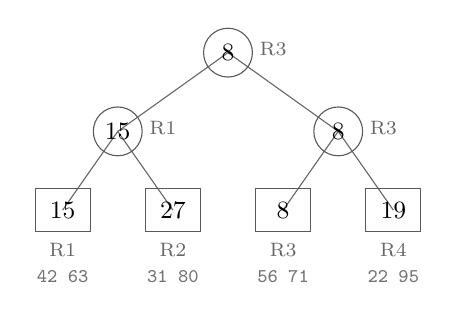
\begin{tikzpicture}[x=0.70cm,y=1.00cm]
\draw[lte] (3,-1) -- (1,-2);
\draw[lte] (3,-1) -- (5,-2);
\draw[lte] (1,-2) -- (0,-3);
\draw[lte] (1,-2) -- (2,-3);
\draw[lte] (5,-2) -- (4,-3);
\draw[lte] (5,-2) -- (6,-3);
\node[ltn] at (3,-1) {$8$};
\node[rlab, anchor=west] at (3.51429,-0.95) {R3};
\node[ltn] at (1,-2) {$15$};
\node[rlab, anchor=west] at (1.51429,-1.95) {R1};
\node[ltn] at (5,-2) {$8$};
\node[rlab, anchor=west] at (5.51429,-1.95) {R3};
\node[ltleaf] at (0,-3) {$15$};
\node[rlab] at (0,-3.5) {R1};
\node[restlab] at (0,-3.85) {42 63};
\node[ltleaf] at (2,-3) {$27$};
\node[rlab] at (2,-3.5) {R2};
\node[restlab] at (2,-3.85) {31 80};
\node[ltleaf] at (4,-3) {$8$};
\node[rlab] at (4,-3.5) {R3};
\node[restlab] at (4,-3.85) {56 71};
\node[ltleaf] at (6,-3) {$19$};
\node[rlab] at (6,-3.5) {R4};
\node[restlab] at (6,-3.85) {22 95};
\end{tikzpicture}
&
\begin{tikzpicture}[x=0.70cm,y=1.00cm]
\draw[lte] (3,-1) -- (1,-2);
\draw[lte] (3,-1) -- (5,-2);
\draw[lte] (1,-2) -- (0,-3);
\draw[lte] (1,-2) -- (2,-3);
\draw[lte] (5,-2) -- (4,-3);
\draw[lte] (5,-2) -- (6,-3);
\node[ltn, ltchg] at (3,-1) {$15$};
\node[rlab, anchor=west] at (3.51429,-0.95) {R1};
\node[ltn] at (1,-2) {$15$};
\node[rlab, anchor=west] at (1.51429,-1.95) {R1};
\node[ltn, ltchg] at (5,-2) {$19$};
\node[rlab, anchor=west] at (5.51429,-1.95) {R4};
\node[ltleaf] at (0,-3) {$15$};
\node[rlab] at (0,-3.5) {R1};
\node[restlab] at (0,-3.85) {42 63};
\node[ltleaf] at (2,-3) {$27$};
\node[rlab] at (2,-3.5) {R2};
\node[restlab] at (2,-3.85) {31 80};
\node[ltleaf, ltnew] at (4,-3) {$56$};
\node[rlab] at (4,-3.5) {R3};
\node[restlab] at (4,-3.85) {71};
\node[ltleaf] at (6,-3) {$19$};
\node[rlab] at (6,-3.5) {R4};
\node[restlab] at (6,-3.85) {22 95};
\end{tikzpicture}
\\[2pt]
{\small (a) 建好之後，冠軍是 $8$（$R_3$）} & {\small (b) 輸出 $8$，$R_3$ 補上 $56$ 後重賽}
\end{tabular}
\diagcaption{勝者樹。 (b) 中橘色的節點是重賽改過的：節點 3 拿 $56$ 和兄弟 $R_4$ 的
$19$ 比，$19$ 贏；節點 1 拿 $19$ 和兄弟節點 2 的贏家 $15$ 比，$15$ 贏。}
\label{fig:lin-winner}
\end{center}

\subsection{敗者樹}
\label{sec:lin-loser}

勝者樹重賽時，每一層都要去讀兄弟節點，才知道要和誰比。 \textbf{敗者樹}（loser
tree，也叫 tree of losers）換個方式記錄：每個內部節點記下那場比賽的\textbf{輸家}，
另外用一個節點 $0$ 記總冠軍。

為什麼記輸家就夠了？ 冠軍從它的葉子一路贏到根。 在路上的節點 $t$，它打敗的是另一
邊子樹的贏家，這位選手就是節點 $t$ 記的輸家。 冠軍的串補上新的鍵後，新鍵沿同一條路
往上重賽，在節點 $t$ 要面對的對手，正是另一邊子樹的贏家，也就是節點 $t$ 記的那位輸
家。 所以每一層只要和\textbf{自己這個節點}記的選手比：贏家繼續往上，輸家留在這個節
點。 走到根之後，留下來的贏家就是新的冠軍，放進節點 $0$。

下面的虛擬碼用 $\mathit{key}[i]$ 表示串 $R_i$ 目前排在最前面的鍵，串讀完了就是
$\infty$。 \proc{Beats}$(a, b)$ 表示串 $a$ 贏串 $b$：$\mathit{key}[a] <
\mathit{key}[b]$，或者兩者相等而 $a < b$（鍵相同時編號小的串贏，這讓合併是穩定
的）。 $L[0..k-1]$ 是敗者樹，$W[1..k-1]$ 只在建樹時暫存每場比賽的贏家。

\begin{pseudo}[label=alg:lin-loser]{敗者樹：由下往上建樹、沿路徑調整}
\Procedure{Build-Loser-Tree}{$k$}
    \For{$t \gets k - 1$ \DownTo $1$}
        \State $a \gets$ 節點 $2t$ 的贏家 \Comment{葉子 $c$ 的贏家是串 $c - k + 1$；內部節點 $c$ 是 $W[c]$}
        \State $b \gets$ 節點 $2t + 1$ 的贏家
        \If{\Call{Beats}{$a, b$}}
            \State $W[t] \gets a$；$L[t] \gets b$
        \Else
            \State $W[t] \gets b$；$L[t] \gets a$
        \EndIf
    \EndFor
    \State $L[0] \gets W[1]$
\EndProcedure
\Procedure{Adjust}{$s$} \Comment{串 $s$ 剛換了新的鍵}
    \State $t \gets \lfloor (s + k - 1) / 2 \rfloor$ \Comment{串 $s$ 的葉子的父節點}
    \While{$t > 0$}
        \If{\Call{Beats}{$L[t], s$}}
            \State 交換 $s$ 和 $L[t]$ \Comment{原本的輸家贏了，往上走；$s$ 留下}
        \EndIf
        \State $t \gets \lfloor t / 2 \rfloor$
    \EndWhile
    \State $L[0] \gets s$
\EndProcedure
\end{pseudo}

\begin{pseudo}[label=alg:lin-kmerge]{用敗者樹做 $k$ 路合併}
\Procedure{K-Way-Merge}{$R_1, \ldots, R_k$}
    \For{$i \gets 1$ \To $k$}
        \State $\mathit{key}[i] \gets R_i$ 的第一個鍵（空的串是 $\infty$）
    \EndFor
    \State \Call{Build-Loser-Tree}{$k$}
    \While{$\mathit{key}[L[0]] \ne \infty$}
        \State $s \gets L[0]$
        \State 輸出 $\mathit{key}[s]$
        \State $\mathit{key}[s] \gets R_s$ 的下一個鍵（讀完了是 $\infty$）
        \State \Call{Adjust}{$s$}
    \EndWhile
\EndProcedure
\end{pseudo}

\textbf{手算追蹤。} 用勝者樹那四個串。 建樹時由下往上：節點 2 是 $R_1$ 的 $15$ 對
$R_2$ 的 $27$，$15$ 贏，記下輸家 $R_2$；節點 3 是 $8$ 對 $19$，記下輸家 $R_4$；節點 1
是兩邊的贏家 $15$ 對 $8$，記下輸家 $R_1$，冠軍 $R_3$ 放進節點 $0$。 建樹比了 $k - 1 =
3$ 次。 之後每輸出一筆，就沿著那個串的葉子往上調整一次。 下圖畫出前三次輸出之後的
樹：方框是節點 $0$ 的冠軍，圓圈是內部節點記的輸家，橘色是這次調整中換了選手的節點，
綠色是剛補上新鍵的葉子。

\begin{center}
\begin{tabular}{c@{\hspace{1.2cm}}c}
\begin{tikzpicture}[x=0.70cm,y=1.00cm]
\draw[lte] (3,-1) -- (1,-2);
\draw[lte] (3,-1) -- (5,-2);
\draw[lte] (1,-2) -- (0,-3);
\draw[lte] (1,-2) -- (2,-3);
\draw[lte] (5,-2) -- (4,-3);
\draw[lte] (5,-2) -- (6,-3);
\draw[lte] (3,-1) -- (3,0);
\node[ltwin] at (3,0) {$8$};
\node[rlab, anchor=west] at (3.51429,0) {R3};
\node[ltn] at (3,-1) {$15$};
\node[rlab, anchor=west] at (3.51429,-0.95) {R1};
\node[ltn] at (1,-2) {$27$};
\node[rlab, anchor=west] at (1.51429,-1.95) {R2};
\node[ltn] at (5,-2) {$19$};
\node[rlab, anchor=west] at (5.51429,-1.95) {R4};
\node[ltleaf] at (0,-3) {$15$};
\node[rlab] at (0,-3.5) {R1};
\node[restlab] at (0,-3.85) {42 63};
\node[ltleaf] at (2,-3) {$27$};
\node[rlab] at (2,-3.5) {R2};
\node[restlab] at (2,-3.85) {31 80};
\node[ltleaf] at (4,-3) {$8$};
\node[rlab] at (4,-3.5) {R3};
\node[restlab] at (4,-3.85) {56 71};
\node[ltleaf] at (6,-3) {$19$};
\node[rlab] at (6,-3.5) {R4};
\node[restlab] at (6,-3.85) {22 95};
\end{tikzpicture}
&
\begin{tikzpicture}[x=0.70cm,y=1.00cm]
\draw[lte] (3,-1) -- (1,-2);
\draw[lte] (3,-1) -- (5,-2);
\draw[lte] (1,-2) -- (0,-3);
\draw[lte] (1,-2) -- (2,-3);
\draw[lte] (5,-2) -- (4,-3);
\draw[lte] (5,-2) -- (6,-3);
\draw[lte] (3,-1) -- (3,0);
\node[ltwin] at (3,0) {$15$};
\node[rlab, anchor=west] at (3.51429,0) {R1};
\node[ltn, ltchg] at (3,-1) {$19$};
\node[rlab, anchor=west] at (3.51429,-0.95) {R4};
\node[ltn] at (1,-2) {$27$};
\node[rlab, anchor=west] at (1.51429,-1.95) {R2};
\node[ltn, ltchg] at (5,-2) {$56$};
\node[rlab, anchor=west] at (5.51429,-1.95) {R3};
\node[ltleaf] at (0,-3) {$15$};
\node[rlab] at (0,-3.5) {R1};
\node[restlab] at (0,-3.85) {42 63};
\node[ltleaf] at (2,-3) {$27$};
\node[rlab] at (2,-3.5) {R2};
\node[restlab] at (2,-3.85) {31 80};
\node[ltleaf, ltnew] at (4,-3) {$56$};
\node[rlab] at (4,-3.5) {R3};
\node[restlab] at (4,-3.85) {71};
\node[ltleaf] at (6,-3) {$19$};
\node[rlab] at (6,-3.5) {R4};
\node[restlab] at (6,-3.85) {22 95};
\end{tikzpicture}
\\[2pt]
{\small (a) 建好之後} & {\small (b) 輸出 $8$，$R_3$ 補上 $56$} \\[10pt]
\begin{tikzpicture}[x=0.70cm,y=1.00cm]
\draw[lte] (3,-1) -- (1,-2);
\draw[lte] (3,-1) -- (5,-2);
\draw[lte] (1,-2) -- (0,-3);
\draw[lte] (1,-2) -- (2,-3);
\draw[lte] (5,-2) -- (4,-3);
\draw[lte] (5,-2) -- (6,-3);
\draw[lte] (3,-1) -- (3,0);
\node[ltwin] at (3,0) {$19$};
\node[rlab, anchor=west] at (3.51429,0) {R4};
\node[ltn, ltchg] at (3,-1) {$27$};
\node[rlab, anchor=west] at (3.51429,-0.95) {R2};
\node[ltn, ltchg] at (1,-2) {$42$};
\node[rlab, anchor=west] at (1.51429,-1.95) {R1};
\node[ltn] at (5,-2) {$56$};
\node[rlab, anchor=west] at (5.51429,-1.95) {R3};
\node[ltleaf, ltnew] at (0,-3) {$42$};
\node[rlab] at (0,-3.5) {R1};
\node[restlab] at (0,-3.85) {63};
\node[ltleaf] at (2,-3) {$27$};
\node[rlab] at (2,-3.5) {R2};
\node[restlab] at (2,-3.85) {31 80};
\node[ltleaf] at (4,-3) {$56$};
\node[rlab] at (4,-3.5) {R3};
\node[restlab] at (4,-3.85) {71};
\node[ltleaf] at (6,-3) {$19$};
\node[rlab] at (6,-3.5) {R4};
\node[restlab] at (6,-3.85) {22 95};
\end{tikzpicture}
&
\begin{tikzpicture}[x=0.70cm,y=1.00cm]
\draw[lte] (3,-1) -- (1,-2);
\draw[lte] (3,-1) -- (5,-2);
\draw[lte] (1,-2) -- (0,-3);
\draw[lte] (1,-2) -- (2,-3);
\draw[lte] (5,-2) -- (4,-3);
\draw[lte] (5,-2) -- (6,-3);
\draw[lte] (3,-1) -- (3,0);
\node[ltwin] at (3,0) {$22$};
\node[rlab, anchor=west] at (3.51429,0) {R4};
\node[ltn] at (3,-1) {$27$};
\node[rlab, anchor=west] at (3.51429,-0.95) {R2};
\node[ltn] at (1,-2) {$42$};
\node[rlab, anchor=west] at (1.51429,-1.95) {R1};
\node[ltn] at (5,-2) {$56$};
\node[rlab, anchor=west] at (5.51429,-1.95) {R3};
\node[ltleaf] at (0,-3) {$42$};
\node[rlab] at (0,-3.5) {R1};
\node[restlab] at (0,-3.85) {63};
\node[ltleaf] at (2,-3) {$27$};
\node[rlab] at (2,-3.5) {R2};
\node[restlab] at (2,-3.85) {31 80};
\node[ltleaf] at (4,-3) {$56$};
\node[rlab] at (4,-3.5) {R3};
\node[restlab] at (4,-3.85) {71};
\node[ltleaf, ltnew] at (6,-3) {$22$};
\node[rlab] at (6,-3.5) {R4};
\node[restlab] at (6,-3.85) {95};
\end{tikzpicture}
\\[2pt]
{\small (c) 輸出 $15$，$R_1$ 補上 $42$} & {\small (d) 輸出 $19$，$R_4$ 補上 $22$}
\end{tabular}
\diagcaption{敗者樹的前三次輸出。 (b)：$56$ 在節點 3 輸給記在那裡的 $19$，$56$ 留下、
$19$ 往上；在節點 1 輸給 $15$，$19$ 留下、$15$ 成為冠軍。 (d)：$22$ 在節點 3 贏
$56$、在節點 1 贏 $27$，一路上都沒有換人，直接成為冠軍。}
\label{fig:lin-loser}
\end{center}

全部十二次輸出列成下表。 「路徑上的比賽」寫出每個節點那場比賽的結果，例如「3：19
勝 56」是在節點 3，$19$ 贏了 $56$；最後一欄是調整完的 $L[0], L[1], L[2], L[3]$。

\begin{center}
\small
\begin{tabular}{ccclc}
\toprule
輸出 & 來自 & 補上的鍵 & 路徑上的比賽（節點：結果） & $L[0..3]$ \\
\midrule
\multicolumn{4}{l}{建樹} & R3 R1 R2 R4 \\
8 & R3 & 56 & 3：19 勝 56；1：15 勝 19 & R1 R4 R2 R3 \\
15 & R1 & 42 & 2：27 勝 42；1：19 勝 27 & R4 R2 R1 R3 \\
19 & R4 & 22 & 3：22 勝 56；1：22 勝 27 & R4 R2 R1 R3 \\
22 & R4 & 95 & 3：56 勝 95；1：27 勝 56 & R2 R3 R1 R4 \\
27 & R2 & 31 & 2：31 勝 42；1：31 勝 56 & R2 R3 R1 R4 \\
31 & R2 & 80 & 2：42 勝 80；1：42 勝 56 & R1 R3 R2 R4 \\
42 & R1 & 63 & 2：63 勝 80；1：56 勝 63 & R3 R1 R2 R4 \\
56 & R3 & 71 & 3：71 勝 95；1：63 勝 71 & R1 R3 R2 R4 \\
63 & R1 & $\infty$ & 2：80 勝 $\infty$；1：71 勝 80 & R3 R2 R1 R4 \\
71 & R3 & $\infty$ & 3：95 勝 $\infty$；1：80 勝 95 & R2 R4 R1 R3 \\
80 & R2 & $\infty$ & 2：$\infty$ 勝 $\infty$；1：95 勝 $\infty$ & R4 R1 R2 R3 \\
95 & R4 & $\infty$ & 3：$\infty$ 勝 $\infty$；1：$\infty$ 勝 $\infty$ & R1 R3 R2 R4 \\
\bottomrule
\end{tabular}
\end{center}

輸出依序是 $8, 15, 19, 22, 27, 31, 42, 56, 63, 71, 80, 95$。 每次調整比 $2 = \lg 4$
次，建樹 $3$ 次，共 $3 + 12 \times 2 = 27$ 次比較。 串讀完時補上 $\infty$，它比任何鍵
都大，自然一路輸到底；兩邊都是 $\infty$ 時照平手的約定，編號小的贏（表中「$\infty$ 勝
$\infty$」）。 所有串都讀完時冠軍的鍵是 $\infty$，合併結束。

\begin{examnote}
敗者樹的追蹤題，每輸出一筆就畫一次整棵樹，內部節點寫輸家（寫鍵，必要時加上串的編
號），另外畫出冠軍（節點 $0$）；只畫冠軍或只列輸出序列都不完整。 鍵相同時誰贏、串讀
完後用 $\infty$ 補，這兩個約定不同課本不一樣，照題目的規定；題目沒說就自己寫明。
\end{examnote}

\textbf{三種做法的比較。} 從 $k$ 個串挑最小，也可以用第~8~章的最小堆積：堆積裡放每
個串目前的鍵，輸出根以後把根換成同一個串的下一個鍵，再做一次下沉。

\begin{center}
\begin{tabular}{p{0.2\linewidth}p{0.22\linewidth}p{0.22\linewidth}p{0.22\linewidth}}
\toprule
 & 勝者樹 & 敗者樹 & 最小堆積 \\
\midrule
節點記什麼 & 每場比賽的贏家 & 每場比賽的輸家，另記冠軍 & 堆積的元素 \\
每輸出一筆的比較次數 & $\lceil \lg k \rceil$ 以內 & $\lceil \lg k \rceil$ 以內 & 最多約 $2\lfloor \lg k \rfloor$ \\
重賽要讀的節點 & 路徑上的節點和它們的兄弟 & 只有路徑上的節點 & 路徑上的節點和兄弟 \\
建立 & $k - 1$ 次比較 & $k - 1$ 次比較 & $O(k)$（第~8~章） \\
\bottomrule
\end{tabular}
\end{center}

堆積下沉時每一層要比兩次（先比兩個子節點，再和較小的比），所以比較次數大約是兩棵
樹的兩倍。 勝者樹和敗者樹比較次數一樣，差在敗者樹重賽時不用讀兄弟節點，每一層只碰
一個節點，程式也比較短，所以外部排序的 $k$ 路合併多半用敗者樹。

\subsection{C 程式}

下面的程式用陣列模擬磁碟上的四個串，\texttt{struct Run} 記錄陣列、長度和下一個要讀
的位置。 為了讓程式短一點，$k$、\texttt{key}、\texttt{L} 和比較次數寫成全域變數。 C 的串編號從 $0$ 開始：串 $i$ 的葉子是節點 $k + i$，父節點是
$(k + i)/2$，正好是虛擬碼的 $\lfloor (s + k - 1)/2 \rfloor$ 把 $s$ 換成 $i + 1$。 印
的時候把編號加 $1$，和上面的圖、表一致。 讀完的串用 \texttt{INT\_MAX} 當 $\infty$，
所以真正的鍵不能是 \texttt{INT\_MAX}。

\begin{example}[label=ex:lin-loser]{c}{(loser\_merge.c) 用敗者樹合併四個串}
#include <stdio.h>
#include <stdlib.h>
#include <limits.h>

// 用陣列模擬磁碟上的一個串，pos 是下一個要讀的位置。
struct Run {
    const int *a;
    int len, pos;
};

int k;             // 串數，串的編號是 0..k-1
int *key;          // key[i]：串 i 目前最前面的鍵，讀完是 INT_MAX
int *L;            // L[1..k-1]：每場比賽的輸家；L[0]：冠軍
long long cmp;     // 比較次數

// 串 a 贏串 b：鍵小的贏，鍵相同時編號小的贏。
int beats(int a, int b)
{
    cmp++;
    return key[a] < key[b] || (key[a] == key[b] && a < b);
}

int next_key(struct Run *r)
{
    return r->pos < r->len ? r->a[r->pos++] : INT_MAX;
}

// 由下往上建樹；w[x] 暫存節點 x 的贏家。葉子 k + i 代表串 i。
void build(void)
{
    int *w = malloc(k * sizeof *w);
    if (w == NULL)
        exit(1);
    for (int x = k - 1; x >= 1; x--) {
        int a = 2 * x >= k ? 2 * x - k : w[2 * x];
        int b = 2 * x + 1 >= k ? 2 * x + 1 - k : w[2 * x + 1];
        w[x] = beats(a, b) ? a : b;
        L[x] = w[x] == a ? b : a;
    }
    L[0] = k > 1 ? w[1] : 0;
    free(w);
}

// 串 s 換了新的鍵：從它的葉子往上，只和每個節點記的輸家比。
void adjust(int s)
{
    for (int x = (s + k) / 2; x > 0; x /= 2) {
        if (beats(L[x], s)) {          // 記在這裡的輸家贏了：交換
            int t = L[x];
            L[x] = s;
            s = t;
        }
    }
    L[0] = s;
}

int main(void)
{
    static const int r1[] = {15, 42, 63}, r2[] = {27, 31, 80},
                     r3[] = {8, 56, 71}, r4[] = {19, 22, 95};
    struct Run runs[] = {{r1, 3, 0}, {r2, 3, 0},
                         {r3, 3, 0}, {r4, 3, 0}};
    k = 4;
    key = malloc(k * sizeof *key);
    L = malloc(k * sizeof *L);
    if (key == NULL || L == NULL)
        return 1;
    for (int i = 0; i < k; i++)
        key[i] = next_key(&runs[i]);
    build();
    printf("build");
    for (;;) {
        printf(" L =");
        for (int x = 0; x < k; x++)
            printf(" R%d", L[x] + 1);  // 印的時候編號從 1 開始
        printf("\n");
        int s = L[0];
        if (key[s] == INT_MAX)         // 冠軍是無限大：全部讀完了
            break;
        printf("out %d R%d", key[s], s + 1);
        key[s] = next_key(&runs[s]);
        adjust(s);
    }
    printf("comparisons = %lld\n", cmp);
    free(key);
    free(L);
    return 0;
}
\end{example}
\iosample{}{build L = R3 R1 R2 R4 \\ out 8 R3 L = R1 R4 R2 R3 \\ out 15 R1 L = R4 R2 R1 R3 \\ out 19 R4 L = R4 R2 R1 R3 \\ out 22 R4 L = R2 R3 R1 R4 \\ out 27 R2 L = R2 R3 R1 R4 \\ out 31 R2 L = R1 R3 R2 R4 \\ out 42 R1 L = R3 R1 R2 R4 \\ out 56 R3 L = R1 R3 R2 R4 \\ out 63 R1 L = R3 R2 R1 R4 \\ out 71 R3 L = R2 R4 R1 R3 \\ out 80 R2 L = R4 R1 R2 R3 \\ out 95 R4 L = R1 R3 R2 R4 \\ comparisons = 27}

每一列的 $L$ 和上面的表一致，總共 $27$ 次比較。 要合併真正的檔案，只要把
\texttt{next\_key} 改成從檔案（經過緩衝區）讀下一個整數，敗者樹的部分不用動。

\subsection{取代選擇：產生更長的初始串}
\label{sec:lin-replace}

合併趟數是 $\lceil \log_k r \rceil$，初始串越少越好。 用內部排序產生初始串，每個串
剛好長 $M$。 \textbf{取代選擇}（replacement selection）在輸出的同時讀入新的紀錄，
平均可以產生長 $2M$ 的串。

想法是這樣：記憶體裡隨時放 $M$ 筆紀錄。 每次輸出記憶體裡最小的那筆到目前的串，空出
來的位置馬上讀入下一筆。 新讀入的鍵如果不比剛剛輸出的小，它還能接在這個串後面；如
果比較小，這個串已經寫過頭了，它只能留給下一個串，稱為\textbf{凍結}。 記憶體裡全部
都凍結時，這個串結束，解除凍結，開始下一個串。

實作上，把每筆紀錄標上它屬於第幾個串，用（串號, 鍵）當堆積的比較依據：串號小的優
先，串號相同時鍵小的優先。 凍結的紀錄串號多 $1$，自然排在目前的串的所有紀錄後面。

\begin{pseudo}[label=alg:lin-replace]{取代選擇}
\Procedure{Replacement-Selection}{$M$}
    \State 讀入前 $M$ 筆紀錄，每筆的串號都設成 $1$
    \State 依（串號, 鍵）把它們建成最小堆積 $H$
    \While{$H$ 不是空的}
        \State $(r, x) \gets H$ 的根
        \State 把 $x$ 寫到第 $r$ 個串的尾端
        \If{輸入還有紀錄}
            \State $y \gets$ 讀入下一筆
            \If{$y \ge x$}
                \State 把根換成 $(r, y)$
            \Else
                \State 把根換成 $(r + 1, y)$ \Comment{凍結，留給下一個串}
            \EndIf
        \Else
            \State 刪掉根，用堆積的最後一筆補上
        \EndIf
        \State 對根做下沉
    \EndWhile
\EndProcedure
\end{pseudo}

\textbf{手算追蹤。} $M = 3$，輸入依序是
\[
41, 17, 63, 29, 8, 52, 35, 12, 70, 24, 58, 6, 47, 33, 90, 15.
\]
每一列是輸出前記憶體裡的三筆（加括號的是凍結的，屬於下一個串）、這一步輸出什麼、補
進來什麼。

\begin{center}
\small
\begin{tabular}{rlccl}
\toprule
步 & 記憶體（輸出前） & 輸出 & 串 & 補進來 \\
\midrule
1 & 41\ \ 17\ \ 63 & 17 & 1 & 29 \\
2 & 41\ \ 29\ \ 63 & 29 & 1 & 8，比 29 小，凍結 \\
3 & 41\ \ (8)\ \ 63 & 41 & 1 & 52 \\
4 & 52\ \ (8)\ \ 63 & 52 & 1 & 35，凍結 \\
5 & (35)\ \ (8)\ \ 63 & 63 & 1 & 12，凍結；全部凍結，串 1 結束 \\
\midrule
6 & 35\ \ 8\ \ 12 & 8 & 2 & 70 \\
7 & 35\ \ 70\ \ 12 & 12 & 2 & 24 \\
8 & 35\ \ 70\ \ 24 & 24 & 2 & 58 \\
9 & 35\ \ 70\ \ 58 & 35 & 2 & 6，凍結 \\
10 & (6)\ \ 70\ \ 58 & 58 & 2 & 47，凍結 \\
11 & (6)\ \ 70\ \ (47) & 70 & 2 & 33，凍結；全部凍結，串 2 結束 \\
\midrule
12 & 6\ \ 33\ \ 47 & 6 & 3 & 90 \\
13 & 90\ \ 33\ \ 47 & 33 & 3 & 15，凍結 \\
14 & 90\ \ (15)\ \ 47 & 47 & 3 & 輸入讀完 \\
15 & 90\ \ (15) & 90 & 3 & --；串 3 結束 \\
\midrule
16 & 15 & 15 & 4 & -- \\
\bottomrule
\end{tabular}
\end{center}

得到四個串：$\langle 17, 29, 41, 52, 63 \rangle$、$\langle 8, 12, 24, 35, 58, 70
\rangle$、$\langle 6, 33, 47, 90 \rangle$、$\langle 15 \rangle$。 用內部排序每次排
$3$ 筆，$16$ 筆會得到 $\lceil 16/3 \rceil = 6$ 個串；取代選擇得到 $4$ 個，前兩個都
比 $M$ 長。 第 2 步的 $8$ 比剛輸出的 $29$ 小，如果讓它進串 1，串 1 就不是排好的了，
所以凍結。

寫成 C 程式時，把虛擬碼~\ref{alg:lin-replace} 的堆積換成第~8~章的陣列堆積，堆積的元
素是（串號, 鍵）的結構，比較時先比串號、再比鍵，其他照抄第~8~章的下沉就可以了。

\textbf{串有多長。} 幾個容易確認的性質：
\begin{itemize}
\item 輸入已經由小到大排好：讀進來的鍵都不比剛輸出的小，永遠不凍結，整個檔案只有一
個串。
\item 輸入由大到小排好：每個新讀入的鍵都比剛輸出的小，全部凍結，每個串剛好 $M$ 筆
（最後一個可能比較短），和內部排序一樣。
\item 一般情況，除了最後一個串，每個串至少 $M$ 筆（觀念題第 10 題）。
\end{itemize}
輸入是隨機的時候，Knuth 證明串的期望長度趨近 $2M$（TAOCP 第 3 卷 5.4.1 節），所以初
始串大約只有 $N/(2M)$ 個，是內部排序的一半。 這裡不證明。

代價是什麼？ 取代選擇每輸出一筆都要做一次堆積調整，$O(\lg M)$，總共 $O(N \lg M)$，
和用內部排序產生初始串同一級；它的串長度不固定，後面的合併程式要能處理長短不一的
串。 實際上也可以用敗者樹代替堆積，比較次數更少。 串長短不一時，先合併哪幾個串會影響總成本；
這和第~19~章的霍夫曼編碼是同一個問題，每次挑最短的 $k$ 個串合併最省。

\textbf{例 2.} 接例 1：$N = 1{,}200{,}000$，$M = 120{,}000$。 用取代選擇，初始串大
約 $N/(2M) = 5$ 個。 $2$ 路合併要 $\lceil \lg 5 \rceil = 3$ 趟（原本 $4$ 趟），$5$ 路
只要 $1$ 趟（原本 $\lceil \log_5 10 \rceil = 2$ 趟）。 總 I/O 次數：$5$ 路合併時是
$150{,}000 \times (1 + 1) = 300{,}000$，比原本的 $450{,}000$ 少三分之一。

\section{本章常見錯誤}
\label{sec:lin-pitfalls}

\begin{center}
\begin{tabular}{p{0.26\linewidth}p{0.48\linewidth}p{0.16\linewidth}}
\toprule
錯誤 & 例子 & 見 \\
\midrule
下界的證明少了一步 & 只寫「葉子數 $\ge n!$」，沒說明不同的順序不能走到同一個葉子 &
第~\ref{sec:lin-lower}~節 \\
以為下界管所有排序 & 「計數排序是 $\Theta(n + k)$，違反了 $\Omega(n \lg n)$ 下界」 &
第~\ref{sec:lin-lower}~節 \\
計數排序從左往右放 & 前綴和之後從 $j = 1$ 開始放，鍵相同的紀錄整個顛倒，不穩定 &
第~\ref{sec:lin-counting}~節 \\
LSD 的方向或穩定性弄錯 & 先排最高位；每一趟用快速排序 & 第~\ref{sec:lin-lsd}~節 \\
趟數忘了取天花板 & $\log_4 10 \approx 1.66$ 寫成 $1.66$ 趟或 $1$ 趟 &
第~\ref{sec:lin-passes}~節 \\
I/O 次數少算一半 & 一趟只算讀，沒算寫；或漏掉產生初始串那一趟 &
第~\ref{sec:lin-passes}~節 \\
敗者樹記成贏家 & 內部節點寫成每場的贏家，那是勝者樹 & 第~\ref{sec:lin-loser}~節 \\
取代選擇沒有凍結 & 新讀入的鍵比剛輸出的小，仍然放進目前的串，串就沒排好 &
第~\ref{sec:lin-replace}~節 \\
\bottomrule
\end{tabular}
\end{center}

\section{觀念題}
\label{sec:lin-exercises}

題型和研究所考試、期中期末考的筆試相近，有選擇、計算、追蹤和證明。 解答在本章最後。

\begin{enumerate}
\item （選擇，可能不只一個答案）下列哪些敘述正確？
\begin{enumerate}
\item 一個正確的比較排序，排 $n$ 個數的決策樹恰好有 $n!$ 個葉子。
\item 合併排序和堆積排序在比較排序裡是漸近最佳的。
\item $n$ 個鍵都是 $0$ 到 $n^2 - 1$ 的整數時，直接用計數排序（$k = n^2 - 1$）就能在
$O(n)$ 時間排好。
\item LSD 基數排序每一趟改用快速排序，結果仍然一定正確。
\item 計數排序的時間可以低於 $n \lg n$，因為它沒有比較鍵的大小，不受比較排序下界的
限制。
\end{enumerate}

\item （追蹤）用選擇排序的想法排三個數 $A[1..3]$：$m \gets 1$；若 $A[2] < A[m]$ 則
$m \gets 2$；若 $A[3] < A[m]$ 則 $m \gets 3$；交換 $A[1]$ 和 $A[m]$；最後若
$A[3] < A[2]$ 就交換 $A[2]$ 和 $A[3]$。 用原本的編號 $a_1, a_2, a_3$ 畫出它的決策樹（鍵兩兩不同）。 樹有幾個葉子？ 哪些葉子
是任何輸入都走不到的？ 最壞和平均各比幾次？

\item （證明）在 $n$ 個兩兩不同的數裡找最大值。
\begin{enumerate}
\item 用決策樹的論證，可以得到什麼下界？
\item 證明任何只用比較的演算法，最壞至少要 $n - 1$ 次比較。
\item 說明為什麼 (a) 的下界和實際差很多。
\end{enumerate}

\item （追蹤）用虛擬碼~\ref{alg:lin-counting} 排序
$A = \langle 2_p, 0_q, 3_r, 2_s, 1_t, 0_u, 2_v \rangle$（$k = 3$，下標的字母是附帶的
資料）。 寫出第 5--6 行做完之後的 $C$，以及第 7--10 行每一輪放完之後的 $B$。

\item （追蹤）六個四位數的編號 $3172, 5408, 1772, 3105, 5472, 1708$。 用 LSD 基數排
序，但以 $100$ 為基底（每「一位」是兩個十進位數字）。 要幾趟？ 寫出每一趟之後的
順序，並指出哪一對編號的最後順序依賴第二趟的穩定性。

\item （計算）桶子排序改用 $m$ 個桶子（$[0, 1)$ 切成 $m$ 等分），輸入仍是 $n$ 個均勻
分布的數。
\begin{enumerate}
\item 求 $E[n_j^2]$，以及第 6 行（插入排序）的總期望時間，用 $n$、$m$ 表示。
\item $m = n/2$ 和 $m = \sqrt{n}$ 時，整個桶子排序的期望時間各是多少？
\end{enumerate}

\item （計算）一個檔案有 $N = 2{,}000{,}000$ 筆紀錄，記憶體放得下 $M = 50{,}000$ 筆，
一個區塊放 $B = 100$ 筆。
\begin{enumerate}
\item 用內部排序產生初始串，有幾個串？
\item 用 $2$ 路、$5$ 路、$8$ 路合併，各要幾趟合併？
\item $8$ 路合併時，包含產生初始串，總共讀寫幾個區塊？
\item 改用取代選擇，以串的期望長度估計，$5$ 路合併要幾趟？
\end{enumerate}

\item （追蹤）用敗者樹合併五個串：
$R_1 = \langle 23, 48 \rangle$、$R_2 = \langle 11, 60, 74 \rangle$、
$R_3 = \langle 35, 39 \rangle$、$R_4 = \langle 17, 52 \rangle$、
$R_5 = \langle 29, 44, 81 \rangle$。 用本章的編號（葉子 $k + i - 1$ 代表 $R_i$）。
\begin{enumerate}
\item 畫出建好的敗者樹，寫出 $L[0..4]$。
\item 畫出輸出兩筆之後的樹。
\item 合併完總共比較幾次？
\end{enumerate}

\item （追蹤）記憶體放得下 $M = 4$ 筆，用取代選擇處理
\[
55, 31, 72, 18, 64, 9, 40, 83, 27, 50, 12, 66, 35, 71, 5, 44,
\]
寫出產生的每個串。 和用內部排序產生初始串相比，串的個數差多少？

\item （證明）證明取代選擇產生的串，除了最後一個，每個都至少有 $M$ 筆。

\item （證明）第~1~章 1.1 節的「找重複學號」。 假設演算法只能問「$a_i = a_j$ 嗎？」（只
能測相等，不能比大小）。 證明在最壞情況下，判斷 $n$ 個數裡有沒有兩個相同，至少要問
$\binom{n}{2}$ 次。（提示：讓對手每次都回答「不相等」。）
\end{enumerate}

\section{實作練習}
\label{sec:lin-practice}

下面是 Aki-Judge 上和本章相關的題目。 這一章的基數排序、敗者樹、取代選擇目前沒有對
應的題目，請以觀念題和本章的範例程式為主。

\begin{center}
\begin{tabular}{llc}
\toprule
小節 & 題目 & 難度 \\
\midrule
計數排序 & \akiref{counting-sort-function}{計數排序函式} & 基本 \\
MSD 基數排序 & \akiref{sort-words-in-dictionary-order}{將單字依字典序排序} & 基本 \\
$k$ 路合併 & \akiref{merge-sorted-number-files-with-counts}{合併排序數列檔並統計次數} & 進階 \\
\bottomrule
\end{tabular}
\end{center}

「計數排序函式」只要交排序函式；鍵的範圍到 $10^6$，計數陣列要用 \texttt{malloc}，
而且這題只有鍵、沒有附帶資料，可以不用輸出陣列 $B$，數完之後直接依序寫回。 「將單字
依字典序排序」可以用 \texttt{qsort} 加 \texttt{strcmp} 通過，練習時試著用
第~\ref{sec:lin-msd}~節的 MSD 基數排序自己寫：依第一個字母分成 $26$ 個桶子，字串
結束的放在最前面的桶子。 「合併排序數列檔並統計次數」是真正讀檔的 $k$ 路合併，每個
檔案同時只保留一個還沒處理的數；$k \le 20$，每次掃過 $k$ 個候選就夠快，想練習的話可
以把範例~\ref{ex:lin-loser} 的敗者樹搬過去。

\section{讀完你應該會}
\label{sec:lin-checklist}

\begin{itemize}
\item 能畫出一個小比較排序的決策樹，用它算最壞和平均的比較次數；能完整寫出比較排序
最壞 $\Omega(n \lg n)$ 的證明，以及平均情況的下界。
\item 能用資訊理論下界和對手論證估計其他問題（插入、合併、找最大值）的比較次數，並
判斷下界是否達得到。
\item 能逐步追蹤穩定的計數排序（前綴和陣列、從右往左放），說明為什麼從右往左才穩定。
\item 能寫出 LSD 基數排序每一趟的結果，說明為什麼內層要穩定，並依位數切法估計成本；能
說明 MSD 和 LSD 的差別、桶子排序期望線性的理由。
\item 給定 $N$、$M$、$B$、$k$，能算出初始串數、合併趟數和 I/O 次數；能比較用內部排序
和取代選擇產生初始串的差別。
\item 能逐步追蹤敗者樹的建立和每次輸出後的調整，並追蹤取代選擇產生的
串。
\end{itemize}

\textbf{延伸閱讀}（書末會整理完整的參考資料）

\begin{itemize}
\item Thomas H. Cormen 等，\textit{Introduction to Algorithms}，第 4 版，第 8 章：決策樹
下界、計數排序、基數排序、桶子排序；章末問題有合併下界、平均下界等延伸。
\item Donald E. Knuth，\textit{The Art of Computer Programming}，第 3 卷第 2 版：5.3.1 節
最少比較次數的排序，5.4.1 節取代選擇與串的期望長度，5.4 節其他小節有多階段合併等外部
排序的方法。
\item Steven S. Skiena，\textit{The Algorithm Design Manual}，第 3 版，第 4 章：排序的
應用和實務上怎麼選排序方法。
\end{itemize}

\addcontentsline{toc}{section}{觀念題解答}
\section*{觀念題解答}

\begin{enumerate}
\item (b)、(e) 正確。 (a)：葉子至少 $n!$ 個，可以更多，例如第 2 題的決策樹有 $8$ 個葉
子，其中兩個走不到。 (c)：計數排序是 $\Theta(n + k) = \Theta(n^2)$；要 $O(n)$ 得用以
$n$ 為基底的基數排序，每個鍵是兩位的 $n$ 進位數，$2$ 趟，每趟 $\Theta(n)$。 (d)：快
速排序不穩定，會破壞前面幾趟的成果，見第~\ref{sec:lin-lsd}~節 $613$、$659$ 的例子。

\item 根是 $1{:}2$（第一個「若」的比較；$a_1 \le a_2$ 往左表示 $m$ 仍是 $1$）。
\begin{itemize}
\item 左子樹（$m = 1$）：比 $1{:}3$。 $a_1 \le a_3$ 時 $m = 1$，不用換，最後比
$2{:}3$，得到 $\langle 1, 2, 3 \rangle$ 或 $\langle 1, 3, 2 \rangle$。 $a_1 > a_3$ 時
$m = 3$，交換後陣列是 $a_3, a_2, a_1$，最後比 $a_1$ 和 $a_2$：$a_2 \le a_1$ 這邊走不
到（已知 $a_1 < a_2$），另一邊交換，得到 $\langle 3, 1, 2 \rangle$。
\item 右子樹（$m = 2$）：比 $2{:}3$。 $a_2 \le a_3$ 時 $m = 2$，交換後陣列是
$a_2, a_1, a_3$，最後比 $a_1$、$a_3$，得到 $\langle 2, 1, 3 \rangle$ 或
$\langle 2, 3, 1 \rangle$。 $a_2 > a_3$ 時 $m = 3$，交換後是 $a_3, a_2, a_1$，最後比
$a_1$、$a_2$：已知 $a_2 < a_1$，所以只走得到 $\langle 3, 2, 1 \rangle$ 那邊，另一邊走
不到。
\end{itemize}
每條路徑都比 $3$ 次，樹有 $2^3 = 8$ 個葉子，其中 $2$ 個走不到，走得到的剛好 $6 = 3!$
個。 最壞、平均都是 $3$ 次，比圖~\ref{fig:lin-dtree} 的平均 $8/3$ 多：這個演算法第三
次比較有時是在問已經知道答案的問題。

\item (a) 答案有 $n$ 種（最大值是哪一個），下界 $\lceil \lg n \rceil$。

(b) 每次比較恰好讓一個數「輸一次」（比較小的那個）。 假設演算法停下來時回答 $z$，
而另外還有一個數 $w \ne z$ 從來沒輸過。 把 $w$ 改成比所有數都大：$w$ 參加過的比較它
本來就都贏，結果不變；其他比較和 $w$ 無關，結果也不變。 演算法看到一樣的結果，仍然回
答 $z$，但現在最大的是 $w$，答錯了。 所以停下來時，除了答案以外的 $n - 1$ 個數都至少
輸過一次，至少要 $n - 1$ 次比較。 從左到右掃一遍剛好用 $n - 1$ 次，所以這個下界是準
的。

(c) 決策樹的論證只用到「答案有 $n$ 種」，每次比較被當成能把可能的答案砍掉一半。 實際
上一次比較最多淘汰一個候選人，砍不了一半，所以資訊理論下界太樂觀。

\item 數完是 $C = [2, 1, 3, 1]$，前綴和之後 $C = [2, 3, 6, 7]$。 從 $j = 7$ 往回放：

\begin{center}
\small
\begin{tabular}{ccl}
\toprule
$j$ & 放到第幾格 & 放完後的 $B[1..7]$ \\
\midrule
7 & 6 & -- -- -- -- -- $2_v$ -- \\
6 & 2 & -- $0_u$ -- -- -- $2_v$ -- \\
5 & 3 & -- $0_u$ $1_t$ -- -- $2_v$ -- \\
4 & 5 & -- $0_u$ $1_t$ -- $2_s$ $2_v$ -- \\
3 & 7 & -- $0_u$ $1_t$ -- $2_s$ $2_v$ $3_r$ \\
2 & 1 & $0_q$ $0_u$ $1_t$ -- $2_s$ $2_v$ $3_r$ \\
1 & 4 & $0_q$ $0_u$ $1_t$ $2_p$ $2_s$ $2_v$ $3_r$ \\
\bottomrule
\end{tabular}
\end{center}
最後的 $C = [0, 2, 3, 6]$，每一格都退到「鍵 $v$ 的第一格的前一格」。

\item 以 $100$ 為基底，四位數是兩「位」，要 $2$ 趟，每趟的計數陣列有 $100$ 格。
第一趟依末兩位（$72, 08, 72, 05, 72, 08$）：$3105, 5408, 1708, 3172, 1772, 5472$。
第二趟依前兩位：$1708, 1772, 3105, 3172, 5408, 5472$。 $1708$ 和 $1772$ 前兩位都是
$17$，第二趟要保持第一趟「$08$ 在 $72$ 前」的順序，靠的是穩定；$3105$ 與 $3172$、
$5408$ 與 $5472$ 也一樣。

\item (a) $n_j$ 是二項分布 $B(n, 1/m)$：$E[n_j] = n/m$，
$\mathrm{Var}[n_j] = \frac{n}{m}(1 - \frac{1}{m})$，所以
$E[n_j^2] = \frac{n}{m}\left(1 - \frac{1}{m}\right) + \frac{n^2}{m^2}$。 $m$ 個桶子加
起來，插入排序的期望時間是
$O\!\left(n\left(1 - \frac{1}{m}\right) + \frac{n^2}{m}\right) = O\!\left(n + \frac{n^2}{m}\right)$。

(b) 整個桶子排序是 $\Theta(n + m) + O(n + n^2/m)$。 $m = n/2$：$O(n)$，仍是線性。
$m = \sqrt{n}$：$O(n^{1.5})$，每個桶子平均有 $\sqrt{n}$ 個數，插入排序在桶子裡變
成平方。

\item (a) $r = \lceil 2{,}000{,}000 / 50{,}000 \rceil = 40$。

(b) $2$ 路：$2^5 = 32 < 40 \le 64$，$6$ 趟。 $5$ 路：$5^2 = 25 < 40 \le 125$，$3$ 趟。
$8$ 路：$8^2 = 64 \ge 40$，$2$ 趟。

(c) 檔案有 $N/B = 20{,}000$ 個區塊，一趟讀寫 $40{,}000$ 次。 產生初始串 $1$ 趟加合併
$2$ 趟，共 $3 \times 40{,}000 = 120{,}000$ 次。

(d) 串的期望長度約 $2M = 100{,}000$，約 $20$ 個串，$5$ 路合併 $\lceil \log_5 20 \rceil
= 2$ 趟，比 (b) 少一趟。

\item (a) $k = 5$，葉子是節點 $5$ 到 $9$：節點 $5, 6, 7, 8, 9$ 依序代表 $R_1$ 到
$R_5$。 節點 $4$ 的子節點是 $8$、$9$，節點 $2$ 的子節點是 $4$、$5$，節點 $3$ 的子節點
是 $6$、$7$。 由下往上：節點 4 是 $17$ 對 $29$，輸家 $R_5$；節點 3 是 $11$ 對 $35$，
輸家 $R_3$；節點 2 是節點 4 的贏家 $17$ 對 $R_1$ 的 $23$，輸家 $R_1$；節點 1 是 $17$ 對
$11$，輸家 $R_4$。 $L[0..4] = R_2, R_4, R_1, R_3, R_5$。

(b) 輸出 $11$（$R_2$ 補 $60$）：節點 3 記的 $35$ 贏 $60$，交換；節點 1 記的 $17$ 贏
$35$，交換；冠軍 $R_4$。 輸出 $17$（$R_4$ 補 $52$）：節點 4 記的 $29$ 贏 $52$，交換；節
點 2 記的 $23$ 贏 $29$，交換；節點 1 記的 $35$ 輸給 $23$，不換；冠軍 $R_1$。 此時
$L[0..4] = R_1, R_3, R_5, R_2, R_4$。

\begin{center}
\begin{tabular}{c@{\hspace{1cm}}c}
\begin{tikzpicture}[x=0.70cm,y=1.00cm]
\draw[lte] (5,-1) -- (3,-2);
\draw[lte] (5,-1) -- (7,-2);
\draw[lte] (3,-2) -- (1,-3);
\draw[lte] (3,-2) -- (4,-3);
\draw[lte] (7,-2) -- (6,-3);
\draw[lte] (7,-2) -- (8,-3);
\draw[lte] (1,-3) -- (0,-4);
\draw[lte] (1,-3) -- (2,-4);
\draw[lte] (5,-1) -- (5,0);
\node[ltwin] at (5,0) {$11$};
\node[rlab, anchor=west] at (5.51429,0) {R2};
\node[ltn] at (5,-1) {$17$};
\node[rlab, anchor=west] at (5.51429,-0.95) {R4};
\node[ltn] at (3,-2) {$23$};
\node[rlab, anchor=west] at (3.51429,-1.95) {R1};
\node[ltn] at (7,-2) {$35$};
\node[rlab, anchor=west] at (7.51429,-1.95) {R3};
\node[ltn] at (1,-3) {$29$};
\node[rlab, anchor=west] at (1.51429,-2.95) {R5};
\node[ltleaf] at (4,-3) {$23$};
\node[rlab] at (4,-3.5) {R1};
\node[restlab] at (4,-3.85) {48};
\node[ltleaf] at (6,-3) {$11$};
\node[rlab] at (6,-3.5) {R2};
\node[restlab] at (6,-3.85) {60 74};
\node[ltleaf] at (8,-3) {$35$};
\node[rlab] at (8,-3.5) {R3};
\node[restlab] at (8,-3.85) {39};
\node[ltleaf] at (0,-4) {$17$};
\node[rlab] at (0,-4.5) {R4};
\node[restlab] at (0,-4.85) {52};
\node[ltleaf] at (2,-4) {$29$};
\node[rlab] at (2,-4.5) {R5};
\node[restlab] at (2,-4.85) {44 81};
\end{tikzpicture}
&
\begin{tikzpicture}[x=0.70cm,y=1.00cm]
\draw[lte] (5,-1) -- (3,-2);
\draw[lte] (5,-1) -- (7,-2);
\draw[lte] (3,-2) -- (1,-3);
\draw[lte] (3,-2) -- (4,-3);
\draw[lte] (7,-2) -- (6,-3);
\draw[lte] (7,-2) -- (8,-3);
\draw[lte] (1,-3) -- (0,-4);
\draw[lte] (1,-3) -- (2,-4);
\draw[lte] (5,-1) -- (5,0);
\node[ltwin] at (5,0) {$23$};
\node[rlab, anchor=west] at (5.51429,0) {R1};
\node[ltn] at (5,-1) {$35$};
\node[rlab, anchor=west] at (5.51429,-0.95) {R3};
\node[ltn] at (3,-2) {$29$};
\node[rlab, anchor=west] at (3.51429,-1.95) {R5};
\node[ltn] at (7,-2) {$60$};
\node[rlab, anchor=west] at (7.51429,-1.95) {R2};
\node[ltn] at (1,-3) {$52$};
\node[rlab, anchor=west] at (1.51429,-2.95) {R4};
\node[ltleaf] at (4,-3) {$23$};
\node[rlab] at (4,-3.5) {R1};
\node[ltleaf] at (6,-3) {$60$};
\node[rlab] at (6,-3.5) {R2};
\node[ltleaf] at (8,-3) {$35$};
\node[rlab] at (8,-3.5) {R3};
\node[ltleaf] at (0,-4) {$52$};
\node[rlab] at (0,-4.5) {R4};
\node[ltleaf] at (2,-4) {$29$};
\node[rlab] at (2,-4.5) {R5};
\end{tikzpicture}
\\[2pt]
{\small (a) 建好之後} & {\small (b) 輸出 $11$、$17$ 之後}
\end{tabular}
\end{center}

(c) 建樹 $k - 1 = 4$ 次。 $R_1$ 的葉子（節點 5）深度 $2$，$R_2$、$R_3$（節點 6、7）深度
$2$，$R_4$、$R_5$（節點 8、9）深度 $3$。 每輸出一筆，就從那個串的葉子往上比一次每一
層：$R_1$ 輸出 $2$ 筆、$R_2$ 輸出 $3$ 筆、$R_3$ 輸出 $2$ 筆，各比 $2$ 次；$R_4$ 輸出 $2$
筆、$R_5$ 輸出 $3$ 筆，各比 $3$ 次。 共 $4 + (2 + 3 + 2) \times 2 + (2 + 3) \times 3 =
33$ 次。 $k$ 不是 $2$ 的次方時，不同的串每次調整的比較次數可能不同。

\item 三個串：$\langle 18, 31, 55, 64, 72, 83 \rangle$、$\langle 9, 12, 27, 35, 40, 50,
66, 71 \rangle$、$\langle 5, 44 \rangle$。 第 2 步輸出 $31$ 後讀入的 $9$、第 3 步輸出
$55$ 後讀入的 $40$ 都凍結；第 6 步輸出 $83$ 後讀入 $50$，記憶體四筆全部凍結，串 1 結
束。 內部排序每次排 $4$ 筆會得到 $16/4 = 4$ 個串，取代選擇少一個，而且前兩個串長
$6$、$8$，都超過 $M$。

\item $N \le M$ 時只有一個串，不用證。 串 $1$ 開始時記憶體是前 $M$ 筆，全部屬於串
$1$。 串 $r \ge 2$ 開始的那一刻，堆積裡最小的串號是 $r$，也就是記憶體裡的紀錄全部屬
於串 $r$。 如果這時記憶體不滿，表示輸入已經讀完，之後不會再讀入紀錄，也就不會出現
串 $r + 1$，串 $r$ 是最後一個。 所以不是最後一個的串，開始時記憶體是滿的，$M$ 筆都
屬於它。 一個串要到記憶體裡沒有它的紀錄才結束，這 $M$ 筆全部會輸出到這個串，所以
它至少有 $M$ 筆。

\item 對手的策略：不管問哪一對，都回答「不相等」。 假設演算法問完不到 $\binom{n}{2}$
次就停下來，那一定有一對 $(i, j)$ 沒問過。 對手手上有兩組都和所有回答一致的輸入：一組
是 $n$ 個兩兩不同的數；另一組只把 $a_j$ 改成和 $a_i$ 一樣，其他不動，這組裡唯一相等的
一對就是沒問過的 $(i, j)$，所以先前每一個「不相等」都仍然成立。 演算法看到同樣的回答，
對兩組輸入給出同樣的答案，但一組沒有重複、一組有，至少錯一組。 所以最壞要問完全部
$\binom{n}{2}$ 對，第~1~章的兩兩比較已經是這個模型裡最好的。 能比大小的話，先排序
（$O(n \lg n)$）再比相鄰的兩個就好；能拿數值當索引的話（查表打勾），只要 $O(n + M)$。
同一個問題，下界取決於演算法被允許問什麼。
\end{enumerate}
